\documentclass[12pt,letterpaper]{article}
\usepackage[utf8]{inputenc}
\usepackage[spanish]{babel}
\usepackage{graphicx}
\usepackage[left=2cm,right=2cm,top=2cm,bottom=2cm]{geometry}
\usepackage{graphicx} % figuras
% \usepackage{subfigure} % subfiguras
\usepackage{float} % para usar [H]
\usepackage{amsmath}
%\usepackage{txfonts}
\usepackage{stackrel} 
\usepackage{multirow}
\usepackage{enumerate} % enumerados
\renewcommand{\labelitemi}{$-$}
\renewcommand{\labelitemii}{$\cdot$}
% \author{}
% \title{Caratula}
\begin{document}

% Fancy Header and Footer
% \usepackage{fancyhdr}
% \pagestyle{fancy}
% \cfoot{}
% \rfoot{\thepage}
%

% \usepackage[hidelinks]{hyperref} % CREA HYPERVINCULOS EN INDICE

% \author{}
\title{Caratula}

\begin{titlepage}
\begin{center}
\large{UNIVERSIDAD PRIVADA-DE-TACNA}\\
\vspace*{-0.025in}
\begin{figure}[htb]
\begin{center}

\includegraphics[width=8cm]{./Imagenes/logo}
\end{center}
\end{figure}
\vspace*{0.15in}
INGENIERIA DE SISTEMAS  \\

\vspace*{0.5in}
\begin{large}
TITULO:\\
\end{large}

\vspace*{0.1in}
\begin{Large}
\textbf{Creando un Reporte Interactivo en Power BI} \\
\end{Large}

\vspace*{0.3in}
\begin{Large}
\textbf{CURSO:} \\
\end{Large}

\vspace*{0.1in}
\begin{large}
Inteligencia de Negocios\\
\end{large}

\vspace*{0.3in}
\begin{Large}
\textbf{DOCENTE(ING):} \\
\end{Large}

\vspace*{0.1in}
\begin{large}
 Patrick Cuadros Quiroga\\
\end{large}

\vspace*{0.2in}
\vspace*{0.1in}
\begin{large}
Integrante: \\
\begin{flushleft}
Jose Luis Condori Choquecota      	\hfill	(2014049088) \\

\end{flushleft}
\end{large}
\end{center}

\end{titlepage}


\tableofcontents % INDICE
\thispagestyle{empty} % INDICE SIN NUMERO
\newpage
\setcounter{page}{1} % REINICIAR CONTADOR DE PAGINAS DESPUES DEL INDICE

\section{Proceso} 

\begin{itemize}
	\item Relacion entre tablas del excel
	\begin{center}
	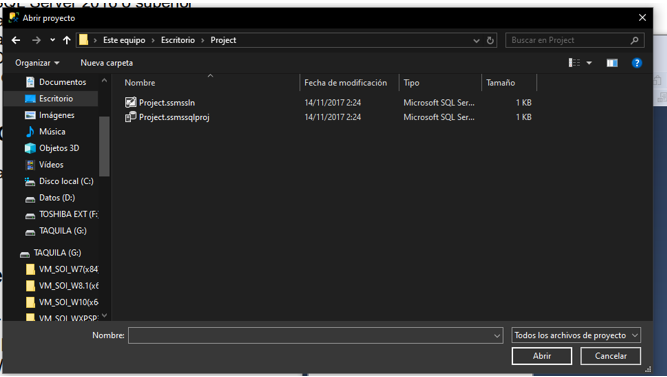
\includegraphics[width=10cm]{./Imagenes/1} 
	\end{center}
\end{itemize} 

\begin{itemize}
	\item Relacion de las tablas despues de agregar el nuevo excel
	\begin{center}
	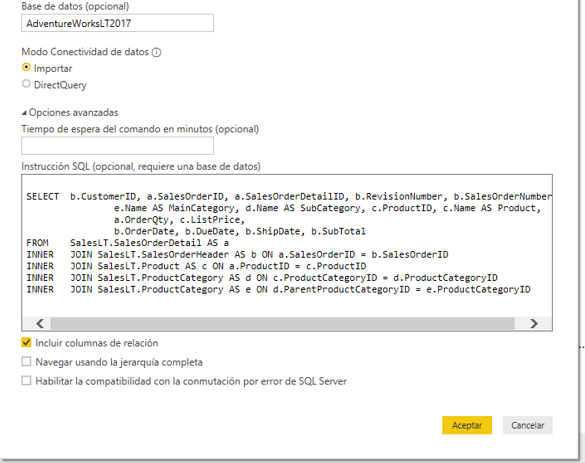
\includegraphics[width=10cm]{./Imagenes/2} 
	\end{center}
\end{itemize} 

\begin{itemize}
	\item Calculo de columna en DimCustomer
	\begin{center}
	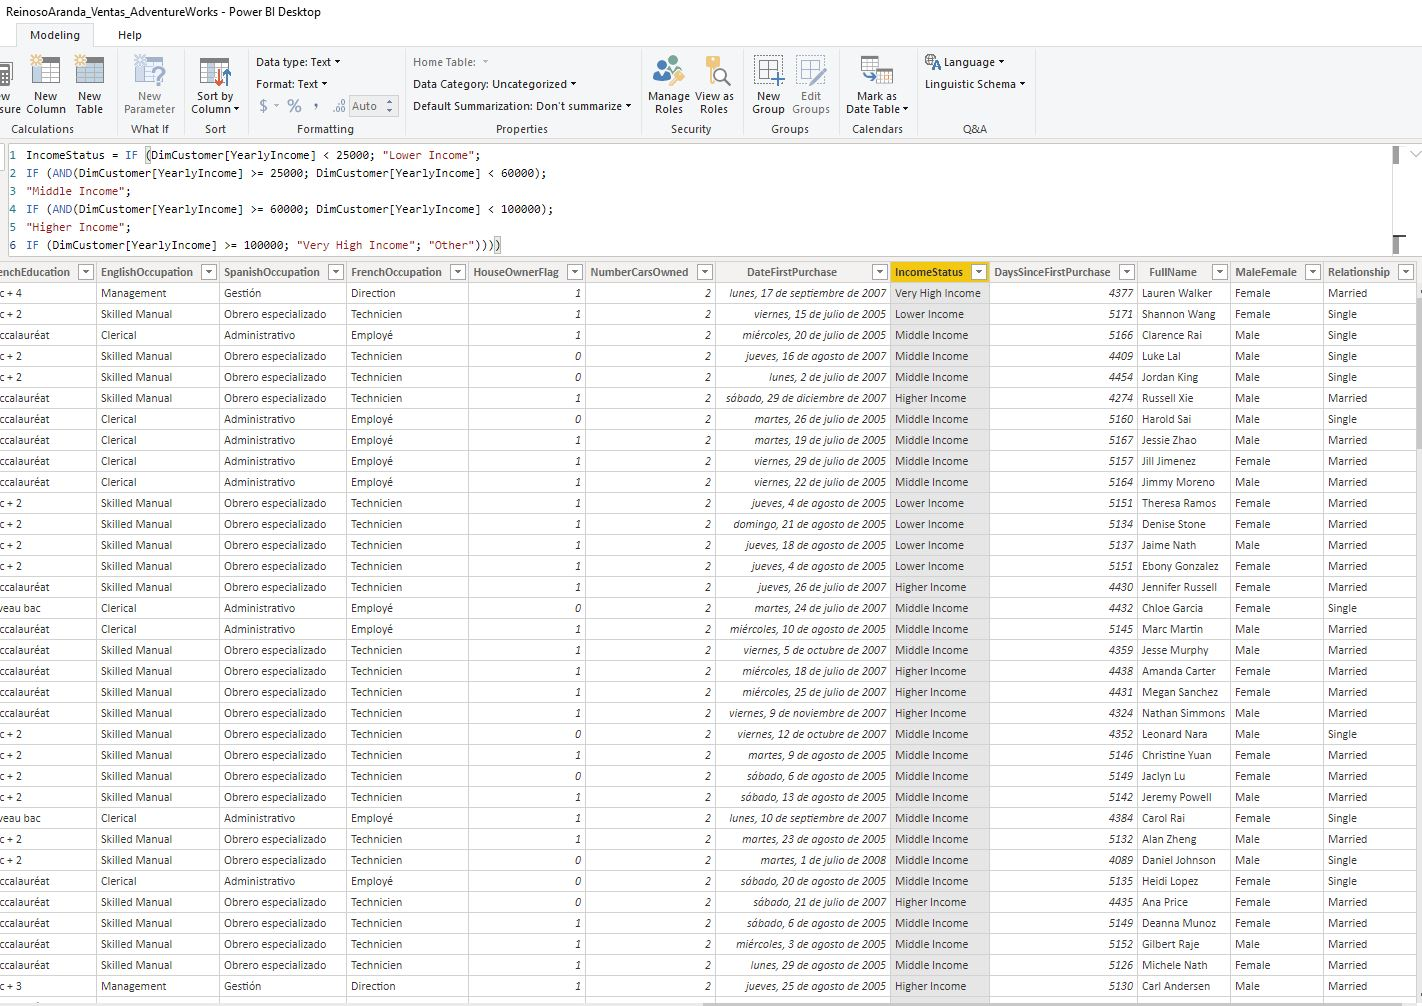
\includegraphics[width=10cm]{./Imagenes/3} 
	\end{center}
\end{itemize} 

\begin{itemize}
	\item Relaciones de las tablas
	\begin{center}
	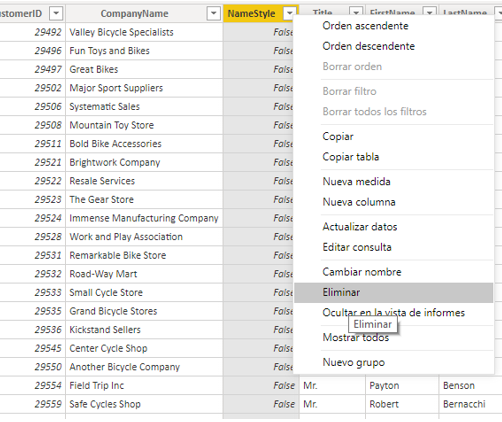
\includegraphics[width=10cm]{./Imagenes/4} 
	\end{center}
\end{itemize} 

\begin{itemize}
	\item Calculo en una columna en la tabla DimProductSubcategory
	\begin{center}
	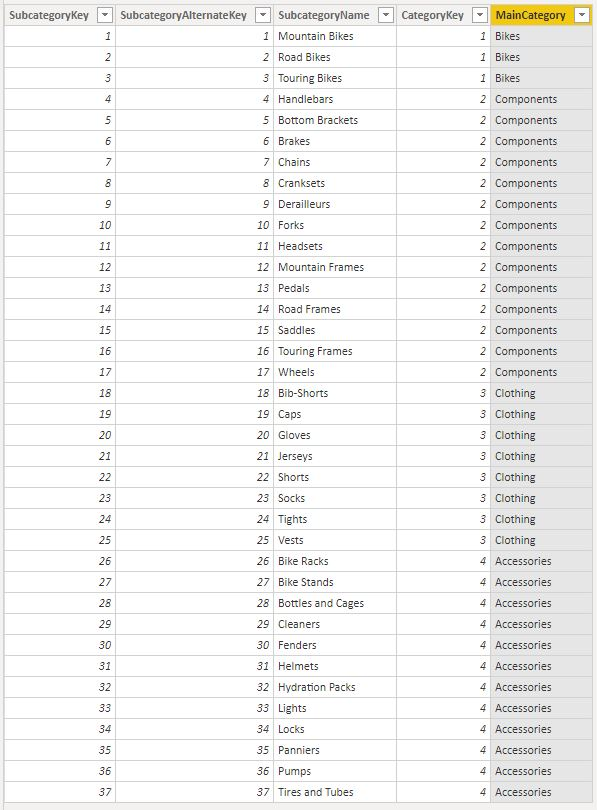
\includegraphics[width=10cm]{./Imagenes/5} 
	\end{center}
\end{itemize} 

\begin{itemize}
	\item Calculo en una columna en la tabla DimPromotion
	\begin{center}
	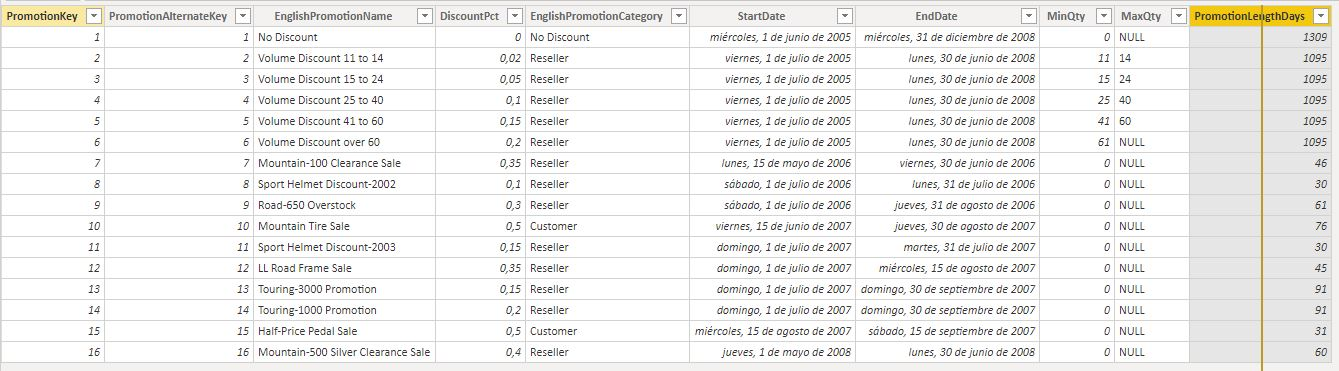
\includegraphics[width=10cm]{./Imagenes/6} 
	\end{center}
\end{itemize} 

\begin{itemize}
	\item Calculo en una columna en la tabla FactInternetSales
	\begin{center}
	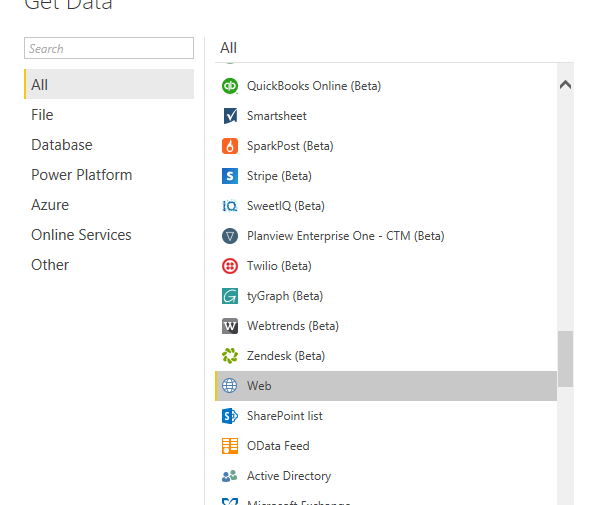
\includegraphics[width=10cm]{./Imagenes/7} 
	\end{center}
\end{itemize} 


\section{Desarrollo}

\begin{itemize}
\subsection{Ejercicio 1:  Conectando a Power BI a datos}\\

\begin{itemize}
\textbf{Tarea 1: Conectar a datos existentes}
\end{itemize} 

\begin{enumerate}
    \item Abrir SQL Server Management Studio, y conectar a la instancia de base de datos (local) utilizando autenticación de Windows.
    
    
    \item En el menú Archivo (File), en el submenu Abrir (Open), hacer click en Project/Solution, y buscar el archivo Project.ssmssln
    
    \begin{center}
	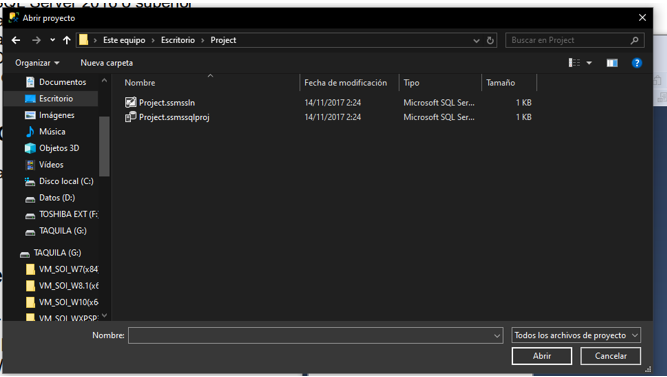
\includegraphics[width=13cm]{./Imagenes/1}
	\end{center}
    
    
    \item En el Explorador de Soluciones, expandir Consultas (Queries), y luego hacer doble click en el archivo Lab Exercise 1.sql.   
    \item Abrir Power BI Desktop.
    
    
    \item En la ventana Power BI Desktop, hacer click en Obtener Data (Get Data).

	
    \item En el cuadro Obtener Datos, click base de datos Microsoft SQL, y entonces click en Conectar
    
    \item En la ventana base de datos Server database, En Servidor, escribir (local).
    
    \item En Base de Datos (opcional), tipear AdventureWorksLT.
    
    
    \item Expandir el cuadro Opciones Avanzadas. Copiar el script Task 1 del archivo Lab Exercise 1.sql. y pegar la consulta en Power BI, en el cuadro sentencia SQL. Luego presionar OK.
    
        \begin{center}
	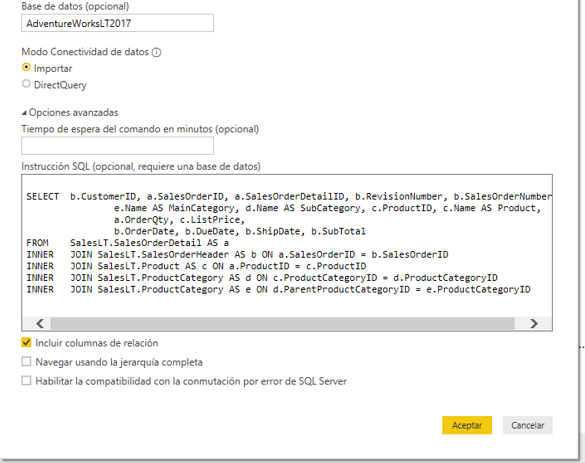
\includegraphics[width=13cm]{./Imagenes/2}
	\end{center}
    
    \item  En la ventana de vista preliminar click en Cargar.
    
    \item En Power BI Desktop, click Obtener Datos y luego click en Mas.

    \item Repetir los pasos del 6 al 10, utilizando el script Task 2.

   \item De regreso en el reporte. Guardar el archivo como AdventureWorksLT Sales.pbix
   
  
\end{enumerate}

\end{itemize}



\begin{itemize}
\textbf{Tarea 2: Graficar Datos}
\end{itemize}

\begin{enumerate}
	\item En el panel Campos (Fields), click derecho sobre Query1, Renombrar, tipear Customers y presionar Enter.
	
    \item Para el Query2, hacer lo mismo del paso 1 y colocar el nombre Sales.
    \item Expandir ambas tablas para ver todas las filas.
    
  
    \item  En la barra de navegación izquierda, haga clic en Datos.
  
    \item En el panel Campos, haga clic en la tabla Clientes, si aún no está seleccionada.
    
    \item Haga clic con el botón derecho en la columna NameStyle y haga clic en Eliminar.

    \begin{center}
	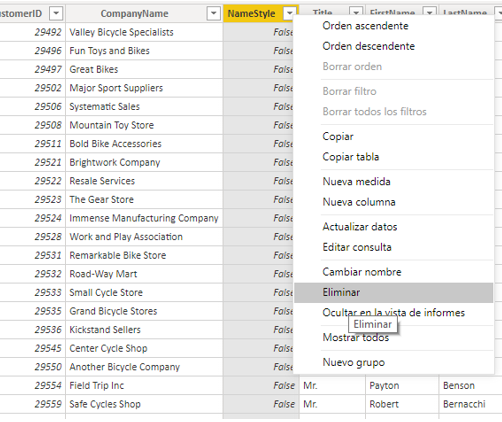
\includegraphics[width=13cm]{./Imagenes/4}
	\end{center}
    \item En el cuadro de diálogo Eliminar columna, haga clic en Eliminar.

    \item Repetir el paso 6 y 7 para la columna SalesPerson.
    
     
    
    \item Haga clic con el botón derecho en la columna CustomerID y luego haga clic en Ocultar en vista de informe.
    
     \item Haga clic en el encabezado de la columna AddressLine1.
    
    \item En la cinta de Modelado, en el grupo Propiedades, haga clic en Categoría de datos: Sin clasificar y luego haga clic en direccion.
    
    
    
    \item Haga clic en el encabezado de la columna Ciudad.
    \item En la cinta de Modelado, en el grupo Propiedades, haga clic en Categoría de datos: Sin clasificar y luego en Ciudad.
     
    \item Haga clic en el encabezado de columna StateProvince. 
    \item En la cinta de Modelado, en el grupo Propiedades, haga clic en Categoría de datos: Sin clasificar y luego haga clic en Estado o Provincia.

    \item Haga clic en el encabezado de columna CountryRegion.
    
    \item En la cinta de Modelado, en el grupo Propiedades, haga clic en Categoría de datos: Sin clasificar y luego haga clic en País / Región

 
    \item Haga clic en el encabezado de columna Código postal.
    \item En la cinta de Modelado, en el grupo Propiedades, haga clic en Categoría de datos: Sin clasificar y luego haga clic en Postal Código.

 
    \item En la cinta de Modelado, en el grupo Cálculos, haga clic en Nueva columna y luego en la barra de fórmulas, escriba
siguiente expresión y presione Entrar:
FullAddress = Clientes [AddressLine1] & "," & Clientes [Ciudad] & "," &
Clientes [StateProvince] & "," & Clientes [CountryRegion] & "," &
Clientes [Código postal]


    \item En el panel Campos, haga clic en Ventas. 
    
    
    
    \item Haga clic con el botón derecho en la columna RevisionNumber y haga clic en Eliminar.
     
    \item En el cuadro de diálogo Eliminar columna, haga clic en Eliminar.
    
    \item Realice el paso 23 y 34 para la columna SalesOrderNumber.
    
    \item Haga clic con el botón derecho en la columna CustomerID y luego haga clic en Ocultar en vista de informe.
    
    
    \item Realice el paso 26 para las columnas SalesOrderID y SalesOrderDetailID.
    
    
    \item En la cinta de Modelado, en el grupo Cálculos, haga clic en Nueva columna y luego en la barra de fórmulas, escriba
siguiente expresión y presione Entrar:
LineTotal = Sales [OrderQty] * Sales [ListPrice]

    \begin{center}
	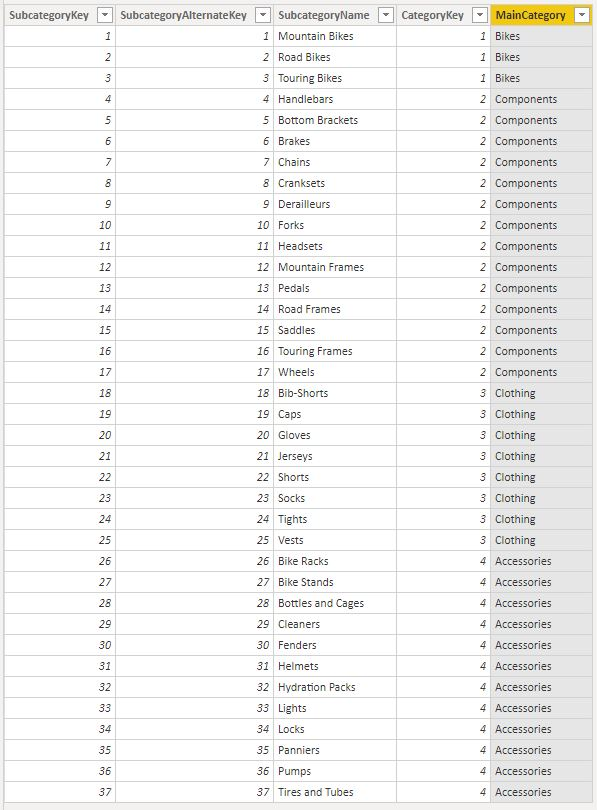
\includegraphics[width=13cm]{./Imagenes/5}
	\end{center}

    \item Haga clic en el encabezado de la columna LineTotal.
    
     
    \item En la cinta de Modelado, en el grupo Formato, haga clic en Formato: General, seleccione Moneda y luego haga clic en Inglés (Estados Unidos).
 
    \item En la cinta de Modelado, en el grupo Cálculos, haga clic en Nueva medida, y luego en la barra de fórmulas, escriba
siguiente expresión y presione Entrar.
TargetSales = SUM ('Ventas' [LineTotal]) * 1.2
    \item Haga clic en Guardar y luego deje abierto Power BI Desktop para la siguiente tarea.
    

\end{enumerate}

\begin{itemize}
\textbf{Tarea 3: Combinar Data
}
\end{itemize}

\begin{enumerate}
	\item En el Explorador de archivos, y luego abra el archivo States.xlsx.
	
    \item En la hoja de trabajo de Estados, seleccione todos los valores en las dos columnas y luego presione Ctrl + C.
    \item En Power BI Desktop, en la cinta de Inicio, haga clic en Introducir datos.
    \item  En el cuadro de diálogo Crear tabla, haga clic en la tabla y luego presione Ctrl + V. Power BI detecta que la primera fila es un encabezado de columna.
    


    \item En el cuadro Nombre, escriba Ventas por estado y luego haga clic en Cargar.
    
        \begin{center}
	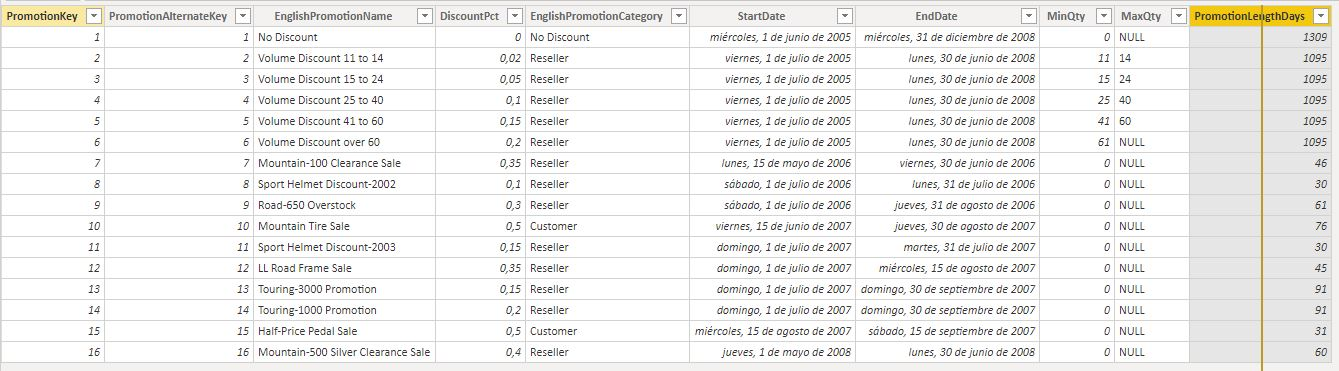
\includegraphics[width=13cm]{./Imagenes/6}
	\end{center}
    
    
    \item En la cinta de Inicio, haga clic en Obtener datos y luego en Web.

    \begin{center}
	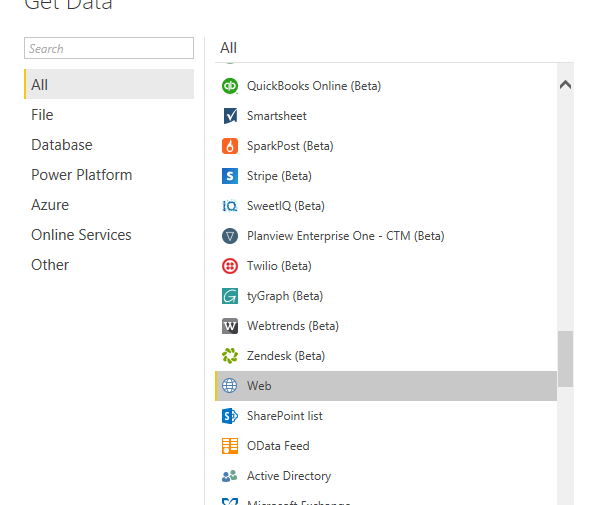
\includegraphics[width=13cm]{./Imagenes/7}
	\end{center}

    \item En el cuadro de diálogo De la web, en el cuadro URL, escriba http://en.wikipedia.org/wiki/List-of-U.S.-state-abbreviations, y luego haga clic en Aceptar.
    
         \begin{center}
	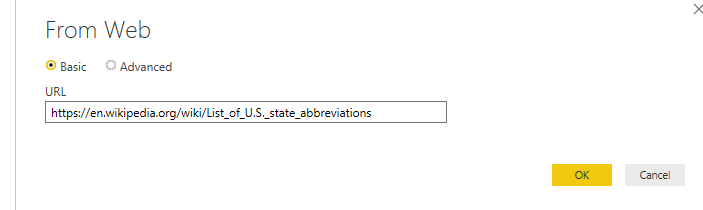
\includegraphics[width=13cm]{./Imagenes/8}
	\end{center}
    
    \item En el cuadro de diálogo Navegador, seleccione Códigos y abreviaturas para estados, territorios y otros Estados Unidos. regiones, y luego haga clic en Cargar.
    
    
     \item En el panel Campos, haga clic en Códigos y abreviaturas para estados, territorios y otras regiones de EE. UU. Para mostrar los datos. La tabla tiene 26 filas en la parte inferior que no son necesarias.
    
    \item En la cinta de Inicio, en el grupo Datos externos, haga clic en Editar consultas, luego haga clic en Editar consultas.
    
    
    
    \item En el Editor de consultas, en el panel Consultas, haga clic en Códigos y abreviaturas para U.S estados, territorios y otras regiones.

     
    \item En la cinta de Inicio, haga clic en Reducir filas, haga clic en Eliminar filas y luego haga clic en Eliminar filas inferiores.
    
    \item En el cuadro de diálogo Eliminar filas inferiores, en el cuadro Número de filas, escriba 26 y luego haga clic en Aceptar.
    
        \begin{center}
	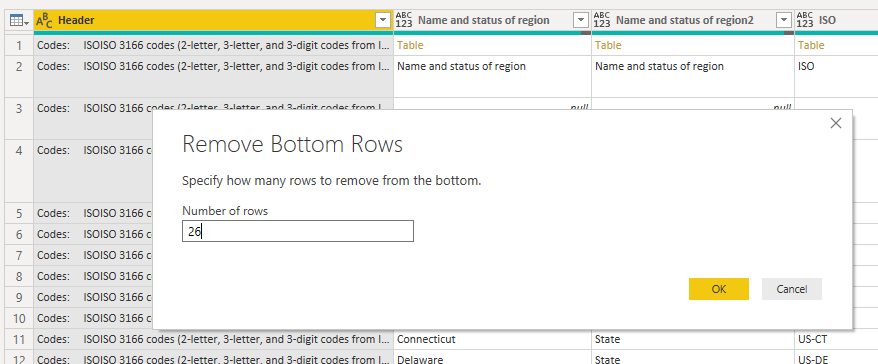
\includegraphics[width=13cm]{./Imagenes/9}
	\end{center}

    \item Haga clic en el encabezado de la columna ANSI2 y luego mantenga presionada la tecla Ctrl mientras selecciona todas las columnas de la derecha. Esto selecciona múltiples filas.
    
    \item Aún manteniendo presionada la tecla Ctrl, haga clic en el Nombre y el estado de las columnas region2 y Encabezado para incluir esto en la selección.

 
    \item En la cinta de Inicio, haga clic en Administrar columnas, haga clic en Eliminar columnas y luego haga clic en Eliminar columnas.
    
    \item En el panel Configuración de consulta, en Propiedades, en el cuadro Nombre, escriba Estados con códigos y luego presione Enter.

 
    \item En la cinta de Inicio, en el grupo Transformar, haga clic en Usar primera fila como encabezados.


    \item Haga clic con el botón derecho en el encabezado de la columna de Estados Unidos de América, haga clic en Cambiar nombre, escriba Nombre del estado y, a continuación, presione Enter.
    
    
    
    \item Haga clic con el botón derecho en el encabezado de la columna US USA 840, haga clic en Cambiar nombre, escriba Código de estado largo y luego presione Enter.
     
    \item Haga clic con el botón derecho en el encabezado de la columna de EE. UU., Haga clic en Cambiar nombre, escriba Código de estado corto y luego presione Enter.
    
    \item En el panel Consultas, haga clic en Ventas por estado.
    
    \item En la cinta de Inicio, haga clic en Combinar y luego en Combinar consultas.
    
    
    \item En el cuadro de diálogo Fusionar, en la tabla Ventas por estado, haga clic en la columna Estados.
    
    
    \item En la lista, haga clic en Estados con códigos, haga clic en la columna Nombre del estado y luego haga clic en Aceptar. La nueva columna es agregado a la tabla y contiene la tabla Estados combinados con códigos.
    \begin{center}
	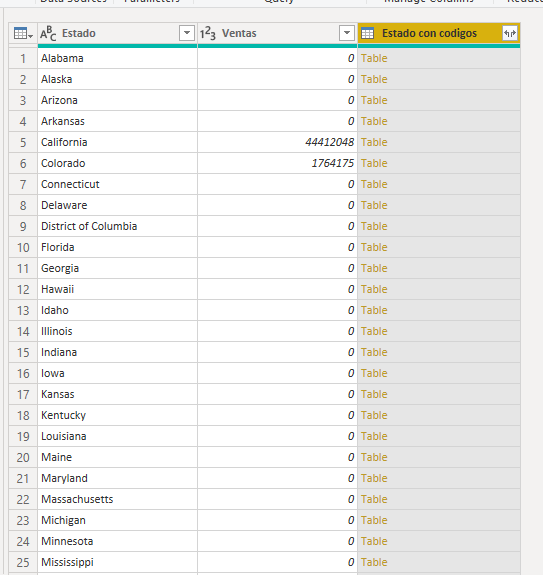
\includegraphics[width=13cm]{./Imagenes/10}
	\end{center}


    \item En el encabezado de la columna, haga clic en el icono Expandir, desactive (Seleccionar todas las columnas), seleccione Código de estado corto, y luego haga clic en Aceptar. La columna ahora muestra solo los códigos de estado.
    
     
    \item Haga clic con el botón derecho en la columna, haga clic en Cambiar nombre, escriba Código de estado y luego presione Enter.
    
    \item En el menú Archivo, haga clic en Cerrar y aplicar.
    
        \begin{center}
	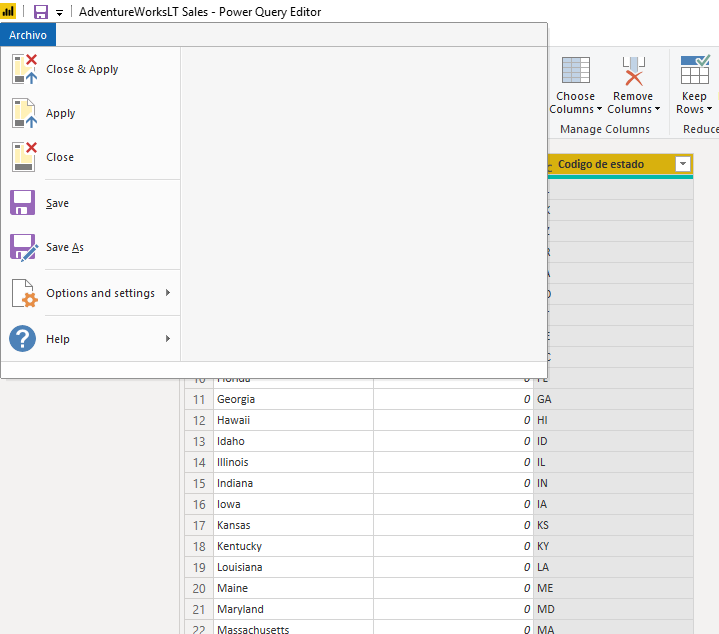
\includegraphics[width=13cm]{./Imagenes/11}
	\end{center}
    
    \item En el panel Campos, haga clic con el botón derecho en Estados con códigos y luego haga clic en Ocultar en vista de informe.
 

    

\end{enumerate}




\subsection{Ejercicio 2:  Construyendo Reportes en Power BI}\\

\begin{itemize}
\textbf{Tarea 1: Crear un Gráfico}
\end{itemize}



\begin{enumerate}

\item En Power BI Desktop, en la barra derecha de navegación, haga clic en Reporte (Informe).

    \item En el panel de Visualizaciones, haga clic en Gauge.

    \item Arrastar el campo LineTotal de la tabla Ventas a la propiedad Valor (Value) del objeto gauge.

    \item Arrastrar la medida TargetVentas de la mesa Ventas a la propiedad Valor destino (valor objetivo) del objeto calibre.
    
    \item Haga clic en Format, exppandir Gauge axis, y luego en el cuadro Max, escriba 146000.
    
    \item Expandir Titulo (Título), en el cuadro Texto de Titulo (Título de texto), tipear Meta de Ventas (Target Sales), y luego haga clic en Centro.


    \item aga clic en el lienzo del informe y luego arrastre el campo CompanyName de la tabla Clientes al informe. Power BI crea automáticamente una tabla.

    \item Arrastar el campo LineTotal de la tabla Ventas en el informe.

    
    \item Asegúrese de que la tabla tenga el foco y luego, en el panel Visualizaciones, haga clic en Gráfico circular.
    
    \item Expanda el gráfico para hacer visibles todos los nombres de las empresas utilizando los controladores de cambio de tamaño en el borde de la tabla.
    
    \item Con el foco aún en el gráfico circular, haga clic en Formato y luego expanda Título.


    \item En el cuadro Texto del título, escriba Clientes más vendidos y luego haga clic en Centro.
    \item EArrastar el campo Categoría principal de la tabla Tabla de ventas en el lienzo del informe. Power BI crea una tabla.
    
    \item Arrastar el campo OrderQty dentro de la tabla.


    \item En el panel Visualizaciones, haga clic en Gráfico de barras apiladas.
    
    \item En el panel Visualizaciones, haga clic en Campos.
    \item Arrastre el campo OrderQty a la propiedad de saturación de color. Tenga en cuenta que los colores cambian.
    
    \item En el panel Visualizaciones, haga clic en Análisis, expanda Línea constante y luego haga clic en Agregar.

    \item En el cuadro Valor, escriba 500.
    
    
    
    
    \item Cambie el color a rojo, cambie la etiqueta Datos a Activado y luego cambie el color a rojo.
    
    \item En el panel Visualizaciones, haga clic en Formato y expanda Título.
    
    \item En el cuadro Texto del título, escriba Pedidos por categoría principal y luego haga clic en Centro.

    \item Haga clic en el lienzo del informe para enfocarlo y luego, en el panel Visualizaciones, haga clic en Gráfico de anillos.
    
    \item En la tabla Ventas, seleccione MainCategory y LineTotal.
    \item En el panel Visualizaciones, haga clic en Formato y luego expanda Título.
    \item En el cuadro de texto Título, escriba Ventas por categoría principal y luego haga clic en Centro.


    \item Arrastre el campo Producto de la tabla Ventas al lienzo del informe. Power BI crea una tabla.
    \item Arrastre el campo LineTotal de la tabla Ventas al gráfico de la tabla de productos.
    
    
    
    
    
    
    
    
    
    
    
    
    
    
 \item En el panel Visualizaciones, haga clic en Campos.
    \item En el panel Filtros, expanda LineTotal (Todos).
    \item En la lista Mostrar elementos cuando el valor, seleccione es mayor que, y luego en el cuadro a continuación, escriba 32000.


    \item Hacer clic en Aplicar filtro (Aplicar filtro).
    \item Expanda MainCategory (All) y luego seleccione Bikes.  
    \item En el panel Visualizaciones, haga clic en Gráfico de columnas apiladas.   
    
    
    
      \item En el panel Visualizaciones, haga clic en Formato y luego expanda Título.
    \item En el cuadro de texto Título, escriba Las 10 bicicletas más vendidas y luego haga clic en Centro.


    \item En el panel Visualizaciones, haga clic en Análisis, expanda Línea constante y luego haga clic en Agregar.
    \item En el cuadro Valor, escriba 35000 y luego configure Color en rojo.  
    \item Cambie la etiqueta de Datos a Activado y luego configure Color en rojo.
    
       \item Expanda el gráfico para llenar el espacio restante en el lienzo del informe. Si es necesario, mueva sus imágenes alrededor para que encajen.  
           \begin{center}
	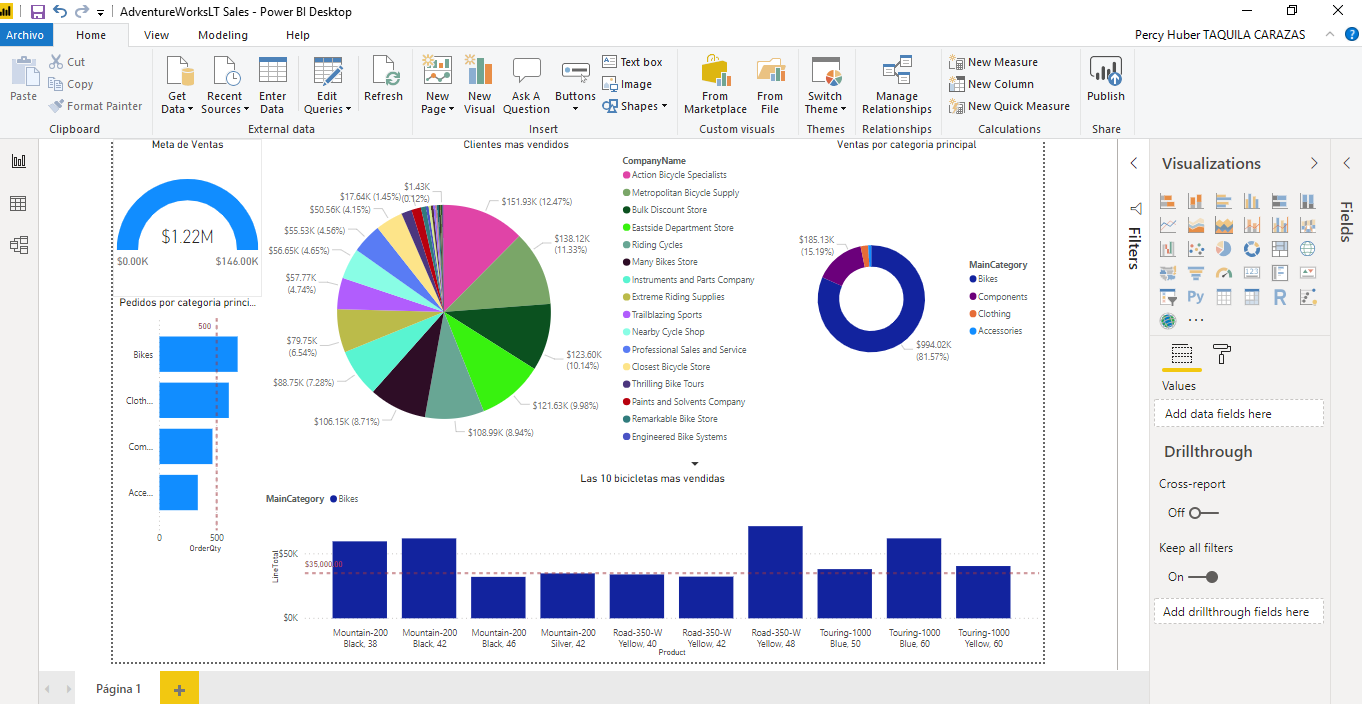
\includegraphics[width=13cm]{./Imagenes/12}
	\end{center}
       
       
       
    \item Haga clic en Guardar
    
    
    


\end{enumerate}



\begin{itemize}
\textbf{Tarea 2: Crear una Visualización de Mapa}
\end{itemize}


\begin{enumerate}

	\item En la parte inferior del informe, haga clic en el ícono + para agregar una nueva página.

    \item En el panel Campos, en la tabla Clientes, seleccione el campo Ciudad. Power BI agrega un mapa al informe.

    \item En el panel Campos, en la tabla Ventas, seleccione el campo LineTotal.
    \item Usando la herramienta de captura en el lado derecho del gráfico, cambie el tamaño del mapa para mostrar todas las burbujas.

    \item Observe que las burbujas tienen un tamaño proporcional para representar los datos.

    \item En el panel Visualizaciones, haga clic en Formato y luego expanda Título.
    
    
    	\item En el cuadro Texto del título, escriba Ventas mundiales por ciudad y luego haga clic en Centro.

    \item Haga clic en el lienzo del informe y luego, en la tabla Ventas por estado, seleccione la columna Código de estado. Power BI agrega automáticamente un mapa.

    \item En la tabla Ventas por estado, seleccione la columna SalesYTD.
    \item En el panel Visualizaciones, haga clic en Mapa lleno. Usando la herramienta de captura en el lado derecho y en la parte inferior de en el gráfico, cambie el tamaño del mapa para mostrar todos los estados.

    \item Observe que las ventas se agrupan en un área.

    \item Coloque el cursor en California (CA) para ver la cifra de ventas. El valor no ha sido formateado como moneda.
    
    	\item En la tabla Ventas por estado, haga clic en la columna SalesYTD

    \item En la cinta de Modelado, seleccione Formato: General, haga clic en Moneda y luego seleccione  Inglés (United Stated).

    \item Posicione el cursor en California (CA) en el mapa y observe que el valor ha sido formateado.
    \item En el panel Visualizaciones, haga clic en Formato y luego expanda Título.

    \item En el cuadro Texto del título, escriba Ventas por estado y luego haga clic en Centro.

    \item Haga clic en Guardar y luego deje el informe abierto para el próximo ejercicio.
Resultados: después de este ejercicio, debería haber creado un informe que tenga gráficos visuales y esté listo para publicar en
el servicio Power BI
    
        \begin{center}
	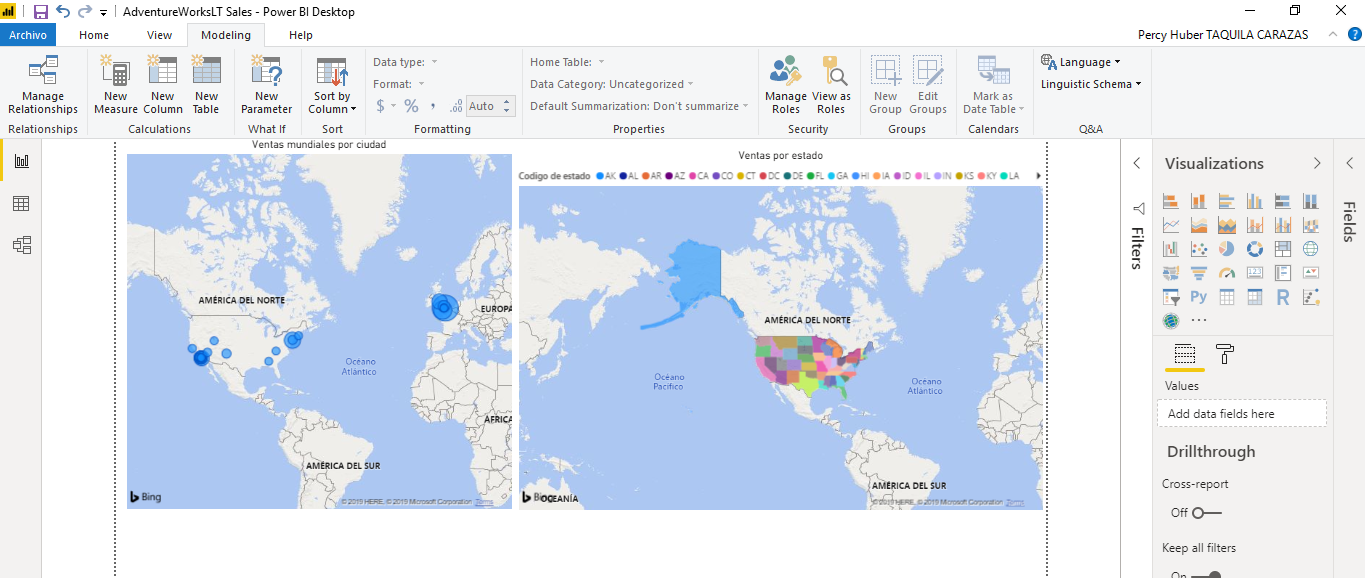
\includegraphics[width=13cm]{./Imagenes/13}
	\end{center}



\end{document}
